\documentclass[conference]{IEEEtran}
\usepackage{cite}
\usepackage{amsmath}
\usepackage{graphicx}
\usepackage{xcolor}
\usepackage[hidelinks]{hyperref}
\usepackage{tikz}
\usetikzlibrary{automata, positioning, arrows.meta}

% Unwritten material is visible rather than missing, so the report is finished
% exactly when no red remains.
\newcommand{\todo}[1]{\textcolor{red}{\textbf{[TODO: #1]}}}

% Marks each section carries, from the brief's marking table. Keeps the effort
% where the marks are.
\newcommand{\weight}[1]{\textcolor{gray}{\small(#1 marks)}}

\begin{document}

\title{Serial Game Server: an authoritative STM32 tic-tac-toe server\\
with a thin PC client}

\author{\IEEEauthorblockN{Tri Tac Le}
\IEEEauthorblockA{LXXTRI004\\Department of Electrical Engineering\\
University of Cape Town}
\and
\IEEEauthorblockN{\todo{partner name}}
\IEEEauthorblockA{\todo{student number}\\Department of Electrical Engineering\\
University of Cape Town}}

\maketitle

\begin{abstract}
\todo{one paragraph: the system, the split of responsibility, and what the
tests demonstrate}
\end{abstract}

\section{Introduction} \weight{10}
\todo{context, the game chosen and why, the GUI library and why, how the work
was split between the two of us, and the shape of this report}

\section{Requirements and message protocol} \weight{15}
The protocol is defined in full in \texttt{docs/protocol.md}.
\todo{bring the command and response table in here, with framing, the board
encoding, and the four departures from the brief called out: NACK:TOOLONG, the
optional player field on MOVE, DISCONNECT from IDLE, and the optional checksum}

\subsection{Framing}
\todo{terminator, the 64 byte maximum, the 2 second partial frame timeout,
what happens to non-printable bytes}

\subsection{Commands and errors}
\todo{the table, plus a sequence diagram of a full game}

\section{Specification and design} \weight{15}
\todo{the server FSM figure, the GUI flowchart and the circuit diagram, all
exported from docs/design.md}

\begin{figure}[htbp]
\centering
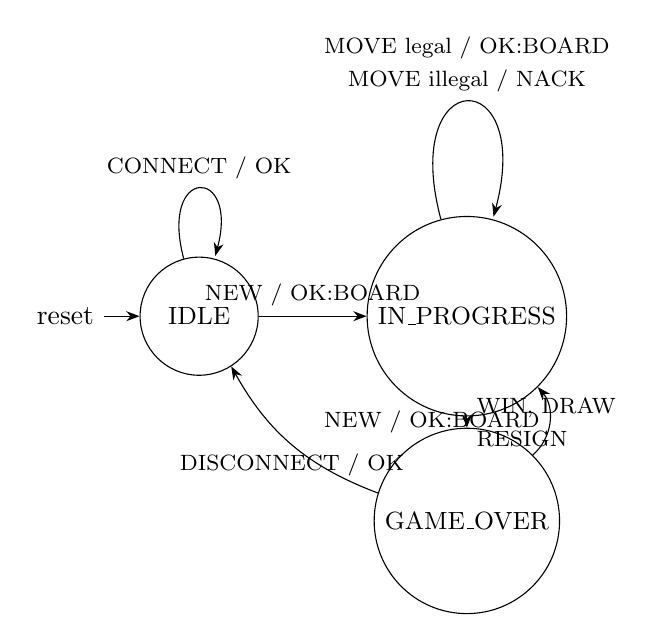
\begin{tikzpicture}[->, >=Stealth, node distance=2.4cm, on grid, auto,
                    every state/.style={draw, minimum size=1.5cm, font=\small}]
  \node[state, initial, initial text={reset}] (idle) {IDLE};
  \node[state, right=3.4cm of idle] (prog) {IN\_PROGRESS};
  \node[state, below=2.6cm of prog] (over) {GAME\_OVER};

  \path
    (idle) edge[loop above] node{\footnotesize CONNECT / OK} ()
    (idle) edge node{\footnotesize NEW / OK:BOARD} (prog)
    (prog) edge[loop above] node[align=center]{\footnotesize MOVE legal / OK:BOARD\\
                                               \footnotesize MOVE illegal / NACK} ()
    (prog) edge node[right, align=left]{\footnotesize WIN, DRAW\\\footnotesize RESIGN} (over)
    (over) edge[bend left=20] node[below]{\footnotesize DISCONNECT / OK} (idle)
    (over) edge[bend right=45] node[left]{\footnotesize NEW / OK:BOARD} (prog);
\end{tikzpicture}
\caption{Server states. Anything a state does not accept is answered
\texttt{NACK:NOGAME} and changes nothing.}
\label{fig:fsm}
\end{figure}

\section{Implementation} \weight{15}
\todo{the excerpts worth explaining: the byte-at-a-time parser and why it never
blocks, the ordering of the move checks, the single 8-bit write to the UART
from interrupt context, and how the same core builds for the board and the
host}

\section{Game logic and server authority} \weight{15}
\todo{validation, turn control, win and draw detection, and the argument that a
rejected request cannot change state, backed by the tests that assert the board
before and after}

\section{Protocol robustness and integrity} \weight{10}
\todo{framing limits, the specific NACKs, recovery from partial and garbage
input, and what the checksum does and does not protect}

\section{Validation} \weight{15}
\todo{the test run output, what each test proves, and screenshots of the GUI
mid-game and after a win}

\begin{table}[htbp]
\caption{Required test cases and where they are covered}
\label{tab:tests}
\centering
\begin{tabular}{p{4.6cm}p{2.6cm}}
\hline
\textbf{Required by the brief} & \textbf{Test} \\
\hline
CONNECT returns OK & \texttt{test\_connect\_returns\_ok} \\
NEW returns an empty board & \texttt{test\_new\_returns\_an\_empty\_board} \\
A legal move changes the board & \texttt{test\_a\_legal\_move\_changes\_the\_board\_exactly} \\
Occupied cell rejected, board unchanged & \texttt{test\_occupied\_cell\_is\_rejected\_and\_nothing\_changes} \\
Out of range rejected & \texttt{test\_out\_of\_range\_is\_rejected} \\
Move after game over refused & \texttt{test\_moves\_after\_game\_over\_are\_refused} \\
Scripted win and draw & \texttt{test\_a\_win\_is\_detected}, \texttt{test\_a\_draw\_is\_detected} \\
\hline
\end{tabular}
\end{table}

\section{Conclusion} \weight{5}
\todo{what works, what it is good for, the limits, and what would be next}

\begin{thebibliography}{1}
\bibitem{brief} University of Cape Town, ``EEE3095S Serial Game Server: CS Project 2026,'' course brief, 2026.
\bibitem{rm0091} STMicroelectronics, ``RM0091 STM32F0x1 reference manual,'' 2021.
\bibitem{tk} Python Software Foundation, ``tkinter: Python interface to Tcl/Tk,'' Python 3 documentation.
\end{thebibliography}

\end{document}
